%%%%%%%%%%%%%%%%%%%%%%%%%%%%%%%%%%%%%%%%%%%%%%%%%%%%%%%%%%%%%%
% ECE 445 SENIOR DESIGN TEMPLATE
%%%%%%%%%%%%%%%%%%%%%%%%%%%%%%%%%%%%%%%%%%%%%%%%%%%%%%%%%%%%%
\documentclass[letterpaper,10pt]{article}

%%%%%%%%%%%%%%%%%%%%%%%%%%%%%%%%%%%%%%%%%%%%%%%%%%%%%%%%%%%%%
% The preamble starts here.
% You can add other packages that you want to use by using
% \usepackage command in the preamble.
% However, DO NOT change the settings that are already placed
% below unless you really know what you are doing.
%%%%%%%%%%%%%%%%%%%%%%%%%%%%%%%%%%%%%%%%%%%%%%%%%%%%%%%%%%%%%

% some commonly used packages
\usepackage{siunitx}
\usepackage{tikz}
\usepackage{listings}
\usepackage{graphicx}
\usepackage{color,soul}
\usepackage{amsmath}
\usepackage{amsthm}
\usepackage{amsfonts}
\usepackage{setspace}
\usepackage{longtable}
\usepackage{url}
\usepackage{pdfpages}
\usepackage{float}
\usepackage{rotating}
\usepackage{caption}
\usepackage{booktabs}  % professional-looking tables
\usepackage{multicol} %used for getting multicolumn without page-break
\usepackage{multirow}	% multi-row tables
\usepackage{array}		% define column format of a table
\usepackage[colorlinks=true,linkcolor=black,citecolor=black]{hyperref}
\usepackage[top=1.1in, bottom=1.1in, left=1.1in, right=1.1in]{geometry}% set the page margins to 1 inch

\lstset{frame=tb,
	language=C,
	aboveskip=3mm,
	belowskip=3mm,
	showstringspaces=false,
	columns=flexible,
	basicstyle={\small\ttfamily},
	numbers=none,
	numberstyle=\tiny\color{gray},
	keywordstyle=\color{blue},
	commentstyle=\color{dkgreen},
	stringstyle=\color{mauve},
	breaklines=true,
	breakatwhitespace=true,
	tabsize=3
}

\usepackage{color}
\definecolor{dkgreen}{rgb}{0,0.6,0}
\definecolor{gray}{rgb}{0.5,0.5,0.5}
\definecolor{mauve}{rgb}{0.58,0,0.82}

% use the fancyhdr package to maintain the format of the page numbers,
% which is useful when the text color is changed
\usepackage{fancyhdr}
\fancyhf{}
\renewcommand{\headrulewidth}{1pt}
\renewcommand{\footrulewidth}{0pt}
\fancyfoot[C]{\textcolor{black}{\thepage}}
\fancyhead[L]{
\includegraphics[width=2cm]{University-of-Illinois-logo.jpg}}
\fancyhead[R]{\small{Infantry I.F.F. Individual Progress Report - Meyers}}

% paralist provides extended list environments
\usepackage{paralist}
\setlength{\plitemsep}{0pt}

% define the color for section and subsection titles
\usepackage{xcolor}
\definecolor{titlecolor}{RGB}{31,73,125}
\definecolor{subtitlecolor}{RGB}{79,129,189}

% change the style of the section and subsection titles
\usepackage{titlesec}
\titleformat{\section}{\color{titlecolor}\Large\bf}{\color{titlecolor}\thesection}{0.8em}{}
\titleformat{\subsection}{\color{subtitlecolor}\large\bf}{\color{subtitlecolor}\thesubsection}{1em}{}
\titleformat{\subsubsection}{\color{subtitlecolor}\normalsize\bf}{\color{subtitlecolor}\thesubsubsection}{1.2em}{}
\titlespacing{\section}{0pt}{0em}{0em}
\titlespacing{\subsection}{6pt}{0em}{0em}
\titlespacing{\subsubsection}{12pt}{0em}{0em}



% change the style of the table of contents
\usepackage{titletoc}
\titlecontents{section}[1.5em]{}{\contentslabel{1.5em}}{\hspace*{-1.5em}}{\titlerule*[0.5pc]{.}\contentspage}
\titlecontents{subsection}[3em]{}{\contentslabel{2.1em}}{\hspace*{-2.1em}}{\titlerule*[0.5pc]{.}\contentspage}
\titlecontents{subsubsection}[5.1em]{}{\contentslabel{2.7em}}{\hspace*{-2.7em}}{\titlerule*[0.5pc]{.}\contentspage}

% command for centering texts in a fixed width table cell
\newcommand{\centpcol}{\leftskip\fill \rightskip\fill}

% command for setting the style of the appendix titles
\newcommand{\setappenstyle}{
	\titleformat{\section}{\color{titlecolor}\Large\bf}{\color{titlecolor}Appendix \Alph{section}}{0.8em}{}
	\titlecontents{section}[0em]{}{Appendix \thecontentslabel \hspace{1em}}{}{\titlerule*[0.5pc]{.}\contentspage}
}

\makeatletter
\newcommand{\skipitems}[1]{%
	\addtocounter{\@enumctr}{#1}%
}

% define the style of the title of the paper
\newcommand{\thetitle}[1]{\title{\begin{huge}{\bf #1}\end{huge} \color{subtitlecolor}\rule[25pt]{\textwidth}{1pt}}}

% define the style of the author
\newcommand{\theauthor}[3]{
	\author{\vspace{.4in}\\
	\textcolor{black}{By}\\
	#1
	\vspace{1in}\\
	\textcolor{black}{ECE 445 Individual Progress Report -} #2\\
	\textcolor{black}{TA:} #3
	\vspace{1in}}
}

% define the style of figure's caption
\newcommand{\figcap}[1]{
	\captionsetup{format=plain,font={small,color=subtitlecolor,singlespacing},margin={0pt,0pt}}
	\caption{\textcolor{subtitlecolor}{#1}}
	\vspace{-5pt}
}

% define the style of table's caption
\newcommand{\tablecap}[1]{
	\captionsetup{format=plain,font={bf,normalsize,singlespacing,color=black},margin={0pt,0pt}}
	\caption{\textcolor{black}{#1}}
	\vspace{-5pt}
}


\newcommand{\buildtoc}{
	\clearpage
	\singlespacing
	\tableofcontents
	\onehalfspacing
}

% set indentations and the space between paragraghs
\setlength{\parindent}{0pt}
\setlength{\parskip}{8pt}

\setcounter{secnumdepth}{4}

\titleformat{\paragraph}
{\normalfont\small\bfseries\color{subtitlecolor}}{\theparagraph}{1em}{}
\titlespacing*{\paragraph}
{18pt}{3.25ex plus 1ex minus .2ex}{1.5ex plus .2ex}

%%%%%%%%%%%%%%%%%%%%%%%%%%%%%%%%%%%%%%%%%%%%%%%%%%%%%%%%%%%%%
% PREAMBLE ENDS HERE, DOCUMENT STARTS BELOW
%%%%%%%%%%%%%%%%%%%%%%%%%%%%%%%%%%%%%%%%%%%%%%%%%%%%%%%%%%%%%

\begin{document}

% don't change these
\pagestyle{empty}
\doublespacing

% put the title of your project here. DO NOT include the brackets.
\thetitle{{I.F.F. (Identification Friend or Foe) System}}

% put your names here. seperate by \\. DO NOT include the brackets.
\theauthor{
	{Noah Prince (nprince2)}\\
}
{ % put the semester info here. DO NOT include the brackets.
	{Spring 2016}
}
{ % put your TA's name here. DO NOT include the brackets.
	{Braedon Salz}
}

% put the date and project number here. DO NOT include the brackets.
\date{
{March 28th, 2016}\\
Project No. 11
\clearpage
}

% don't change these
\maketitle
\pagestyle{fancy}
\begin{spacing}{1.15}


% build the table of contents. 
\color{black}
\buildtoc
\pagenumbering{gobble}
\clearpage
\setcounter{page}{1}
\pagenumbering{arabic}

%SECTION - Introduction
\section{Introduction}
\subsection{Overview}
The team is building an infantry IFF (Identification Friend or Foe) system. Such a system will notify infantry units when their firearm is pointed at a friendly target. Specifically, this system will mount on a firearm and flash green when pointed at a friendly. The firearm mount is referred to in this report as the interrogator unit. Another system, the target unit, will mount on the chest of infantry units and other non-combatant/friendlies. 

The interrogator unit broadcasts a unique id(identification) via a laser transmitter. The target unit, upon receipt of a unique id, broadcasts an acknowledge signal via an isotropic radio transmitter. 

\subsection{Personal Involvement}
With the clear division of friendly target and friendly interrogator, it made sense for the team to divide work amongst these modules. Over the past 8 weeks, I have worked on the schematics/pcb layout for the friendly target unit along with the laser broadcast and the laser receiver. 

These accomplishments are detailed below:
\begin{itemize}
	\item Circuit Schematic \& PCB for Friendly Target Unit
	\item Circuit Schematic \& PCB for KH3 Radio Transmitter Breakout Board
	\item Research into Laser Strength, Safety, Lenses and Construction
	\item Appropriate Laser Parts Ordered
	\item Appropriate Photodiode Acquired
	\item Basic LED Broadcast and Photodiode Receiver Circuit 
\end{itemize}

%SECTION - Design
\section{Design}

%DESIGN - FRIENDLY INTERROGATOR UNIT
\subsection{Overview} \label{section-friendly-interrogator-design}
One may refer to the figure in the Design Review of this project labeled "Block Diagram of Friendly Target Unit" to get a high-level understanding of how the friendly target unit functions. 

\subsection{Calculations}
The majority of the calculations required for this project were already performed in the design review. This includes laser safety and effective reception distance, as well as power and radio calculations. Eric worked on the radio calculations, while I worked on the laser and photodiode calculations. 

One calculation that was not included in the Design Review is the one for an adjustable focus laser. The original intention was to buy a pre-made adjustable focus laser. This was, for the required distances, impossible. Instead, the scope of the project has changed to include building a custom adjustable focus laser. 

The laser is still limited to 5mW. The calculations in the following section give a baseline for the adjustable focus. 

\subsubsection{Adjustable Focus Calculations}
Adjustable focus is achieved by placing a convex lens in series after a concave lens. The convex lens is generally on a screw so that unscrewing increases the distance between the lenses. The effective focus of the dual-lens system can be described by 

\begin{center}
	\large
	$f = \frac{1}{f_1} + \frac{1}{f_2} - \frac{d}{f_1 f_2}$
\end{center}

Where $f$ is the effective focus, $f_1$ is the focal length of the concave lens (negative), $f_2$ is the focal length of the convex lens (positive) and $d$ is the distance between the lenses. 

Furthermore, the required focal length for this project can be described as 

\begin{center}
	\large
	$f = \frac{w}{Tan(\theta)}$
\end{center}

Where $w$ is the beam width and $\theta$ is the divergence of the beam. In the scope of this project, 

\begin{center}
	\large
	$Tan(\theta) = \frac{r}{D}$
\end{center}

Where $D$ is the distance to the target, and $r$ is the radius of the beam at that distance. 

Following from these equations, 

\begin{center}
	\large
	$f = \frac{Dw}{r} =  \frac{1}{f_1} + \frac{1}{f_2} - \frac{d}{f_1 f_2}$
\end{center}

This setup requires a tube, a laser, both lenses, and some a screwing cap for the tube. With their varying price and relative cheapness, PVC pipes and caps were a clear choice. 

PVC pipe caps have $\frac{1}{2}$ inches of screwing distance. The beam width for the laser is around $2mm$. The spot radius is $20cm$. In order to test indoor in close quarters (i.e. the lab), the fully unscrewed distance should reach a spot radius of $20cm$ at $20 m$. This diverges slightly from the closest requirement of $50m$, but will still be able to hit $20cm$ at $50m$ and will make debugging easier. Fully screwed, the spot radius should be $20cm$ at $300m$. This gives two equations with two unknowns: 

\begin{center}
	\large
	$\frac{300*.002}{0.2} =  \frac{1}{f_1} + \frac{1}{f_2} - \frac{0}{f_1 f_2}$ \\
	$\frac{20*.002}{0.2} =  \frac{1}{f_1} + \frac{1}{f_2} - \frac{0.0127}{f_1 f_2}$
\end{center}

Solving these equations
\begin{center}
	\large
	$f_1 \approx -53mm$ \\
	$f_2 \approx  52mm$
\end{center}

Unfortunately, the best lenses that I could find with matching diameters (for the PVC pipe) were $-51mm$ and $50mm$, respectively. This gives a far distance of $255 m$ and a close distance of $18.6131 m$. This will likely lead to a shift in requirements later in the semester. 
%Subsection - Preliminary Breadboard Testing
\subsection{Preliminary Breadboard Testing}
This section contains descriptions of breadboard testing of modules that I have performed or plan to perform.

\subsubsection{Photodiode}
The schematic presented in the design review uses 4 photodiodes, all with equivalent circuits. To test the photodiode signal processing circuit, I built a single photodiode circuit on a breadboard. The operational amplifier was powered by a power source at +/- 12V. A function generated was used in a transistor circuit to pulse an LED next to the photodiode. An oscilloscope was placed on the output of the amplified photodiode signal on the operational amplifier. 

After eliminating ground loops and debugging the circuit, I was able to find a resistor value (500k) that ensured a signal ranging from 0 to 3.3V. 

\subsubsection{R.F. Transmitter and Receiver}
In order to test the Linx KH3 transmitter and receiver (surface mount boards) on a breadboard, two "breakout" boards were created. The modules can be soldered to these breakout boards, which route all pins on the boards to breadboard-compatible pin headers. These breakouts are detailed in the PCB schematics. 

The testing procedure was as follows: Place both units on a breadboard. Power the modules via an external power source at 3.3V. Route all address bits on both units to ground. Route arbitrary values to the data bits on the transmitter. Wire LEDs to all output signals on the receiver. Set TE to high on the transmitter. Ensure the data LEDs on the receiver display the arbitrary values sent from the transmitter. 

Unfortunately, in initial breadboard testing, I accidentally inverted the receiver board pins. When hooked to a power source, the receiver started smoking and never functioned after. As such, we have ordered another receiver and will test it after spring break. 

%Subsection - Circuit Schematics
\subsection{Circuit Schematics} \label{section-circuit-schematics}

\subsubsection{Friendly Interrogator Unit}
The friendly target unit has five major modules: the AAT217 DC-DC step-up converter, the PDM1-S DC-DC 3.3V to +/- 12V converter, the photoreceiver unit, the R.F. transmitter, and the MCU. 

Please refer to Eric's individual progress report or the design review for more information on the AAT217 DC-DC step-up converter; as he worked on this system.
 
The schematics are displayed below.
\begin{figure} [H]
	\centering
	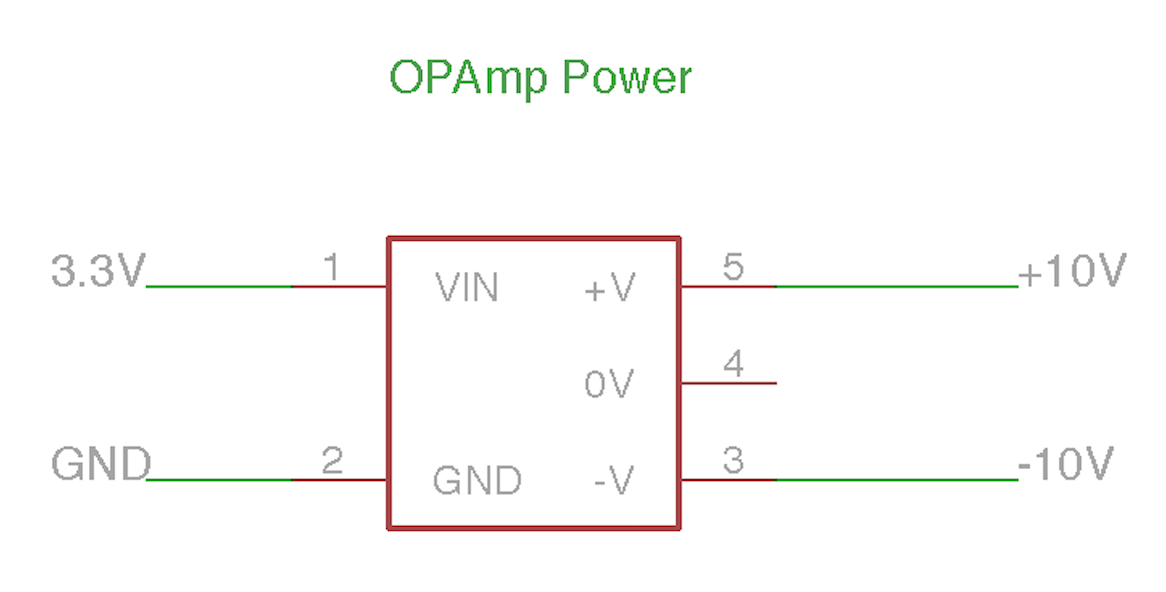
\includegraphics[scale=0.35]{opamp-power.png}
	\caption{PDM1-S DC-DC 3.3V to +/- 12V Converter (Op Amp Power Circuit) Schematic \label{fig:voltage-converter-schematic}}
\end{figure}

\begin{figure} [H]
	\centering
	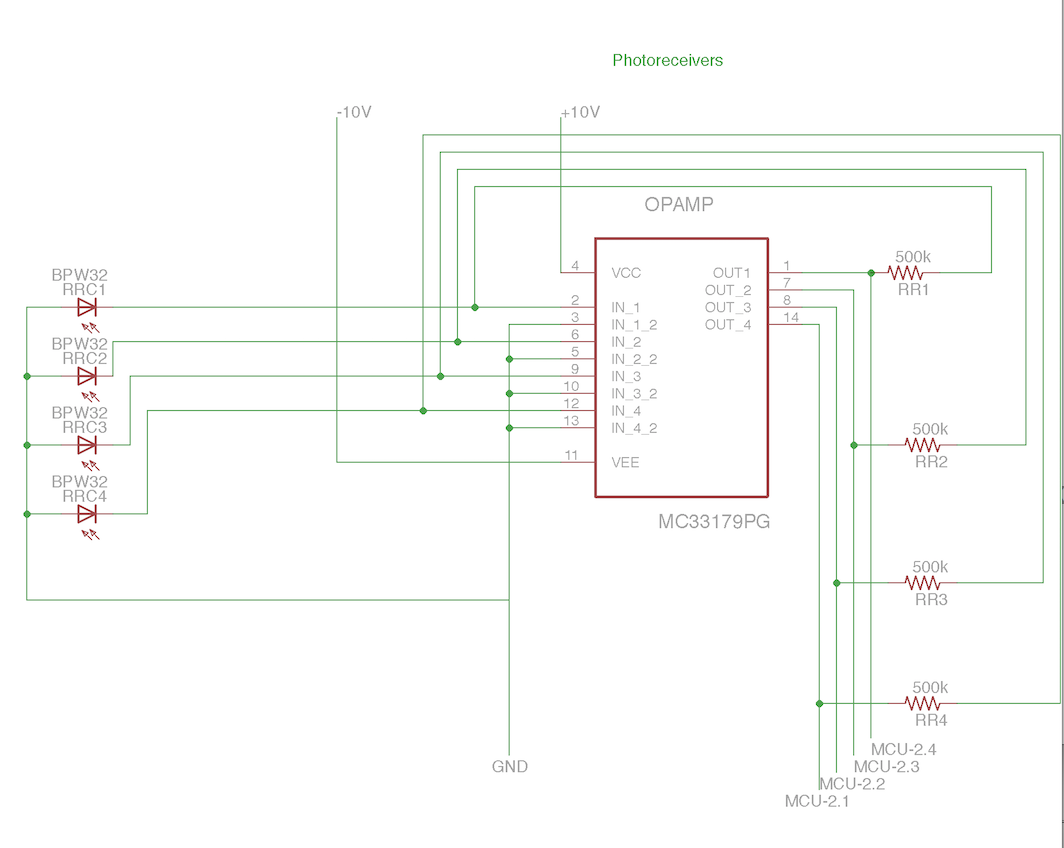
\includegraphics[scale=0.7]{photoreceiver.png}
	\caption{Photoreceiver Schematic \label{fig:photoreceiver-schematic}}
\end{figure}

\begin{figure} [H]
	\centering
	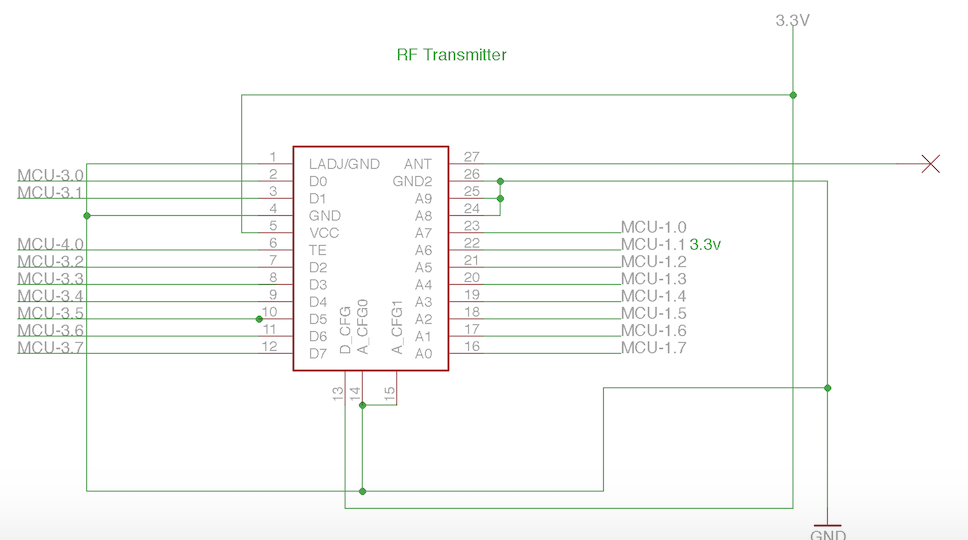
\includegraphics[scale=0.70]{rf-transmitter.png}
	\caption{R.F. Transmitter Schematic \label{fig:transmitter-schematic}}
\end{figure}

\begin{figure} [H]
	\centering
	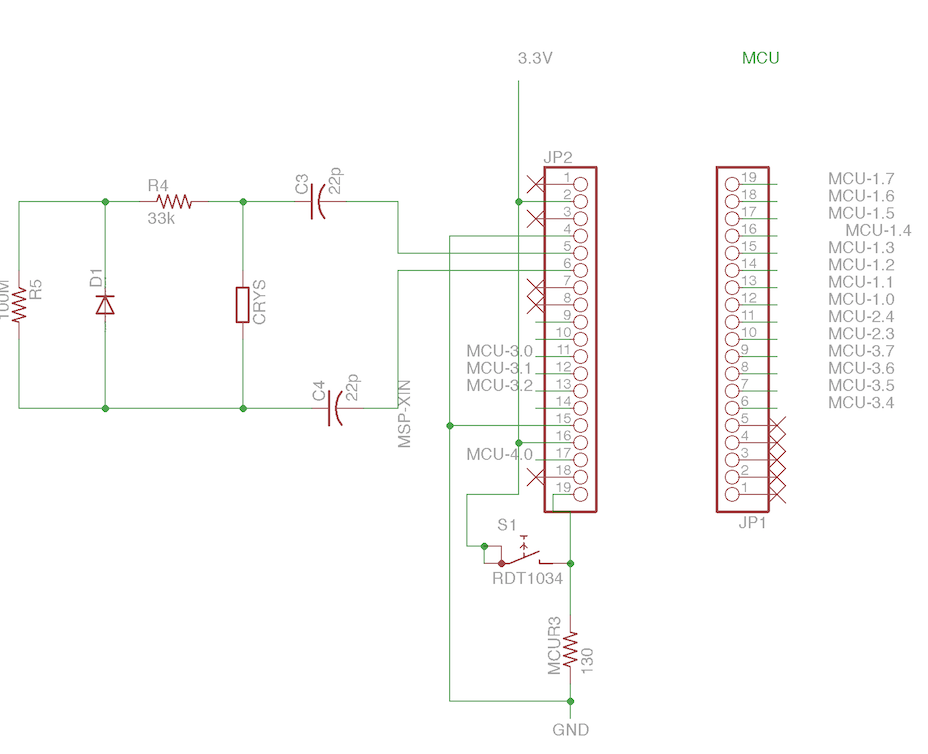
\includegraphics[scale=0.75]{mcu.png}
	\caption{MCU Schematic\label{fig:msp-schematic}}
\end{figure}


\subsubsection{System PCB Schematic}
Shown below in Figure \ref{fig:system-pcb} is the initial PCB schematic of the friendly target unit. This will be used for debugging; we will likely order a final PCB chip to iron out any bugs. 

\begin{figure} [H]
	\centering
	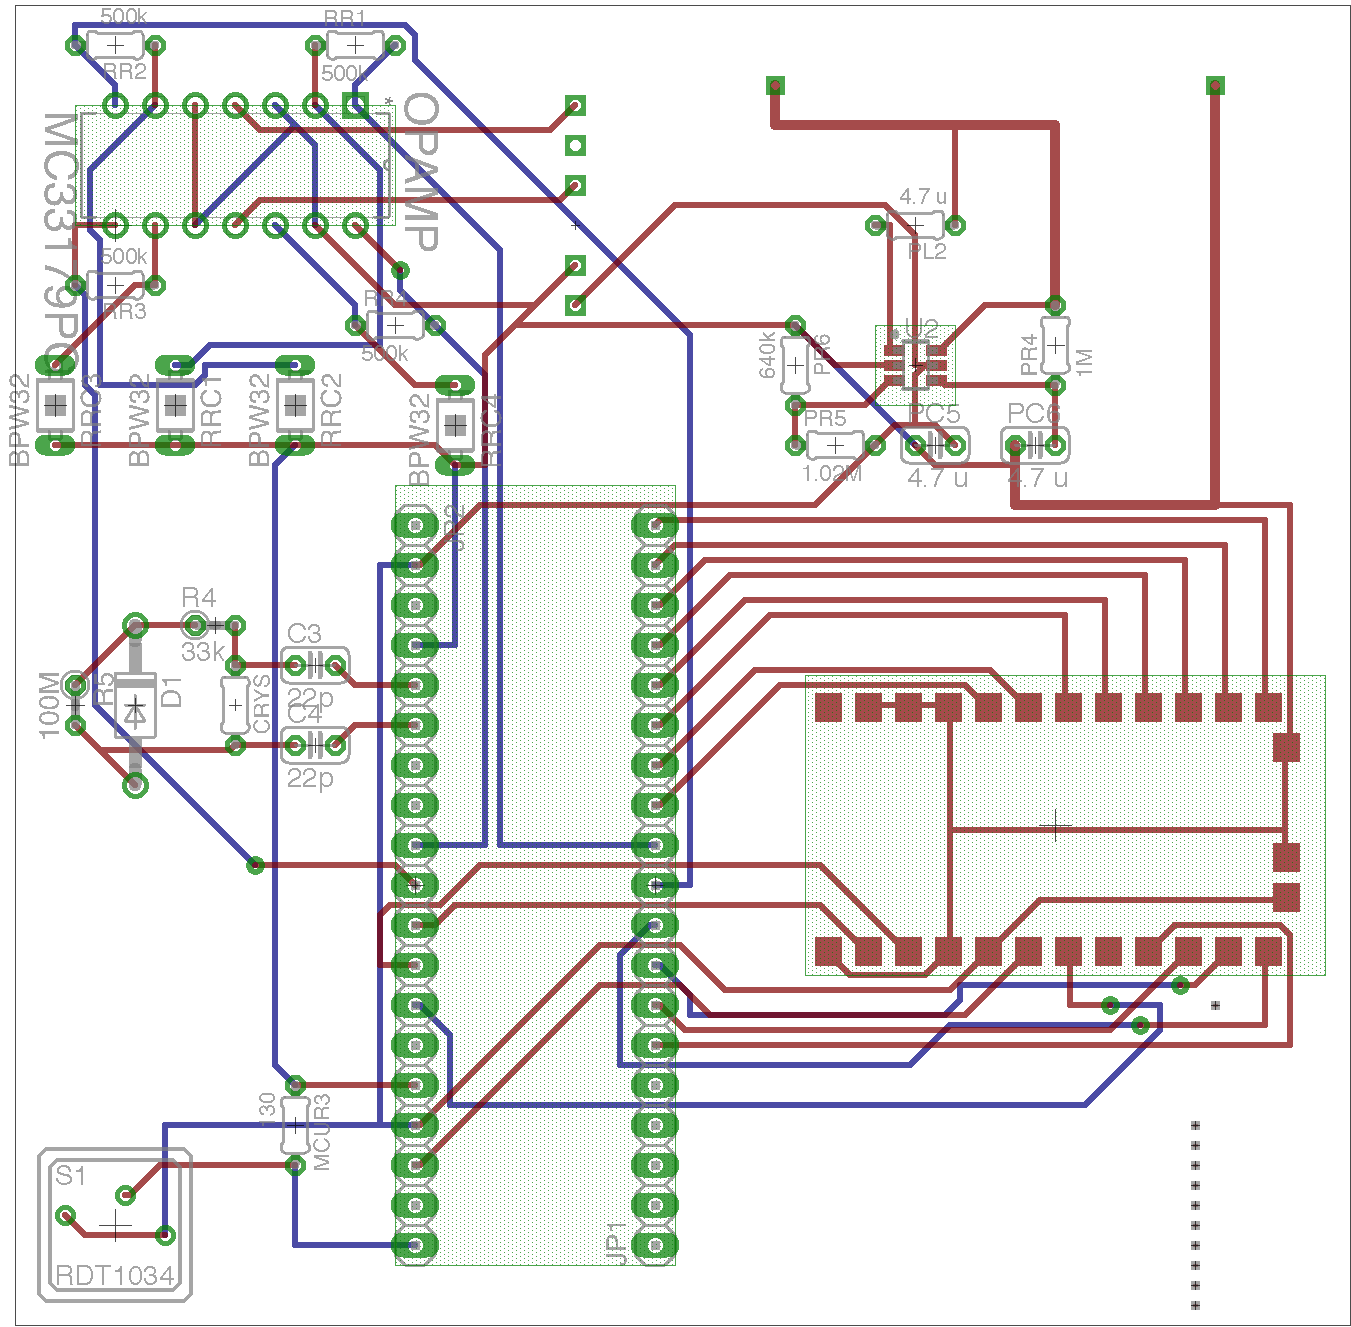
\includegraphics[scale=1.5]{system-pcb.png}
	\caption{Overall System PCB Schematic\label{fig:system-pcb}}
\end{figure}

\subsubsection{PCB Sub-Schematics and Verification}
See Eric's individual progress report for more information on the MSP430 breakout and mounting. Eric's progress report also contains information on the voltage converter PCB layout. Debugging will be similar on both boards, even though the layout may be different. 

The PDM1-S DC-DC 3.3V to +/- 12V converter, the photoreceiver unit and the R.F. transmitter are essential to successful operation of the target unit. Below is an descriptions of each module, along with an inflated view of the module on the PCB. The descriptions include debugging and requirement verification strategies. 

\normalsize\textbf{PDM1-S DC-DC 3.3V to +/- 12V converter}\\
This converter steps up the 3.3V output from the AAT217 DC-DC step-up converter to +/- 12V for use in the photoreceiver. The photoreceiver uses operational amplifiers which require a high voltage to boost the photodiode signal.

The points -12V and +12V will be probed with a digital multimeter upon receiving 3.3V on the bottom most pin.  

The verification of this unit will happen after the AAT1217 has been soldered to the board and verified. 1.5V will be supplied to the AAT1217, which will then supply 3.3V to this converter. Upon verification, the photoreceiver unit will be soldered and verified.
\begin{figure} [H]
	\centering
	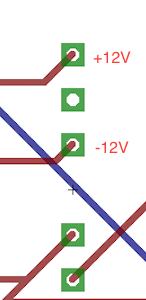
\includegraphics[scale=0.8]{12vconverter.png}
	\caption{+/- 12V Converter PCB Schematic\label{fig:converter-pcb}}
\end{figure}

\normalsize\textbf{Photoreceiver} \\
The photoreceiver will receive the 40kHz pulsed id from the laser on the interrogator unit. 

For each photoreceiver output, corresponding to the 4 available photodiodes, the verification will be as follows: Pulse a laser aimed at the photodiode at a 75\% duty cycle. Attach an oscilloscope to the output of the photoreceiver (labeled Out 1-4 in Figure \label{fig:photodiode-pcb}). Verify the output is a 75\% duty cycle wave on the oscilloscope. 

Note that this verification will be performed with the laser within 5 cm of the photodiode; this will cause the photoreceiver to output near it's maximum voltage. The team will verify that the voltage output from each photoreceiver output does not exceed 3.3V. 

This verification will take place after the +/-12V converter is soldered. This will ensure the operational amplifier has sufficient voltage. Once this component is soldered and verified, the MCU will be soldered and verified. 
\begin{figure} [H]
	\centering
	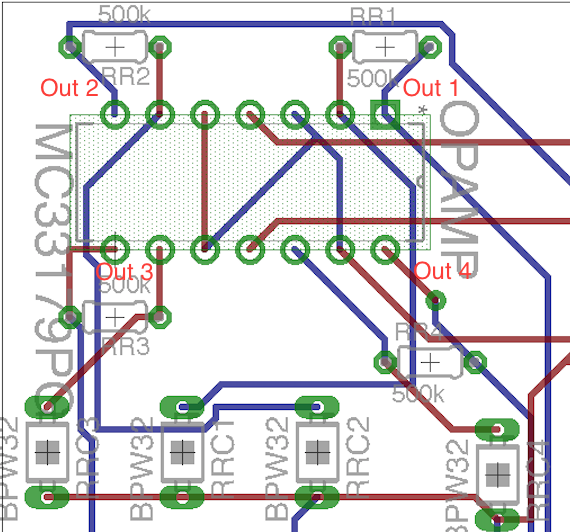
\includegraphics[scale=1]{photoreceiver-pcb.png}
	\caption{Photoreceiver PCB Schematic\label{fig:photodiode-pcb}}
\end{figure}

\normalsize\textbf{MCU} \\
The MCU will control the Linx KH3 transmitter and will receive signal input from the photoreceiver unit. 

After the pcb is powered up, the team will write basic software to test the MCU. This software will likely 1) read from the 4 photoreceiver outputs with a pulsing laser hitting them (similar to the test for the photoreceiver unit) and 2) output address and data bits to the R.F. transmitter on the pcb, which will be verified by a digital multimeter. The team will also verify 3) that the MCU can receive signal from the "sync" button and 4) keep a valid clock. These can all be verified with software and a multimeter. 

This verification will be performed after the photoreceiver is verified. Upon verification, the R.F. transmitter will be soldered and verified. 
\begin{figure} [H]
	\centering
	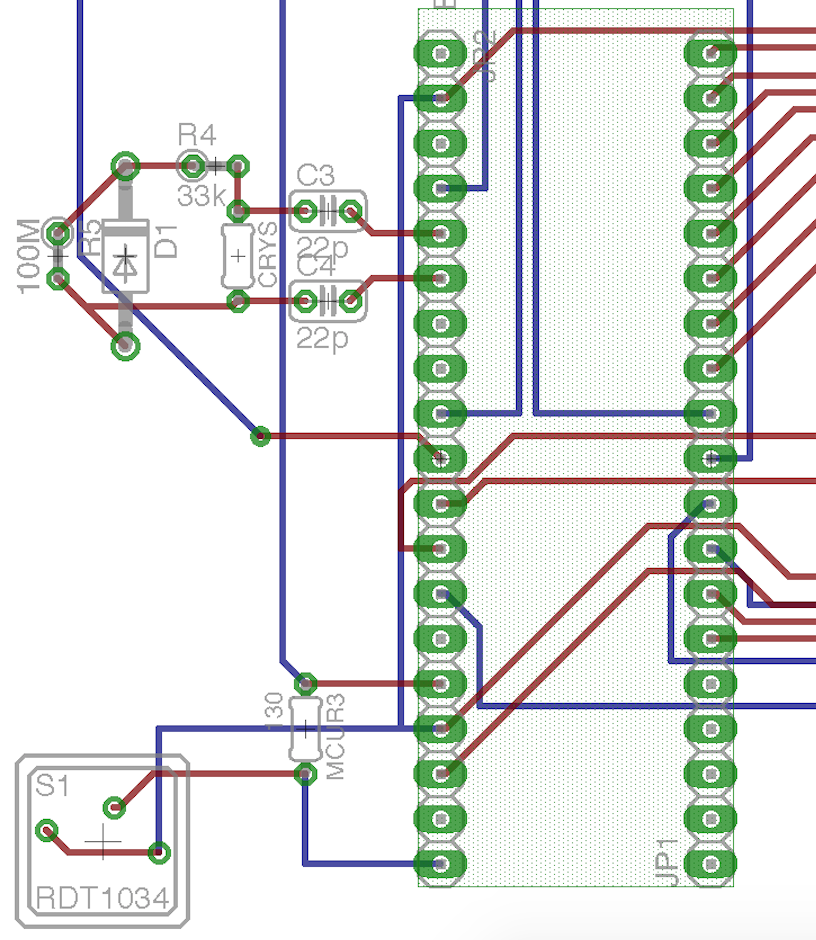
\includegraphics[scale=.7]{mcu-pcb.png}
	\caption{MCU PCB Schematic\label{fig:mcu-pcb}}
\end{figure}

\normalsize\textbf{R.F. Transmitter} \\
This module will transmit the friendly "ack" signal to the interrogator unit. 

This module is dependent on the R.F. Receiver module, and as such they will be tested and verified as a pair. 

Prior to soldering either unit to the pcb, they will both be verified (together) on a PCB. This will ensure both parts are functioning as intended. The breadboard testing setup is described in section \label{section:radio-breadboard}. The R.F. transmitter, then, will be detached from the breadboard and soldered to the PCB. The receiver will remain connected and powered on the breadboard.

Similar to the breadboard testing, the MCU will be programmed to set all address bits to ground and all data bits to an arbitrary pattern consisting of ground and 3.3V. TE will then be set to high. I will ensure the LEDs attached to the receiver on the breadboard accurately display the arbitrary pattern. 

With the completion of this verification, the PCB will be ready for software debugging. 
\begin{figure} [H]
	\centering
	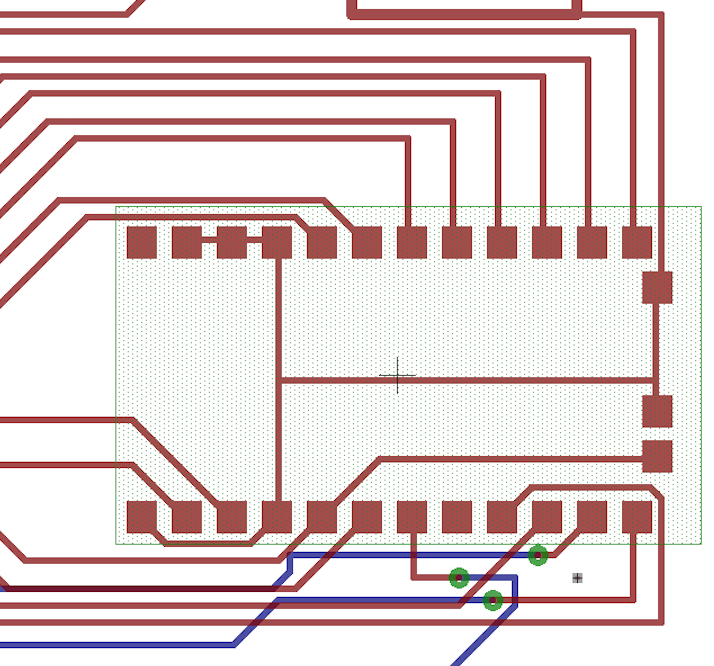
\includegraphics[scale=0.8]{rf-transmitter-pcb.png}
	\caption{R.F. Transmitter PCB Schematic\label{fig:rf-transmitter-pcb}}
\end{figure}

The KH3 transmitter and receiver must first be tested to verify that it is properly functioning before soldering to the friendly interrogator PCB. For this reason a breakout board to be used in conjunction with a breadboard was created to test. This is shown below in Figure \ref{fig:transmitter-breakout} and Figure \ref{fig:receiver-breakout}. The transmitter breakout was created by myself, the receiver by Eric.

\begin{figure} [H]
	\centering
	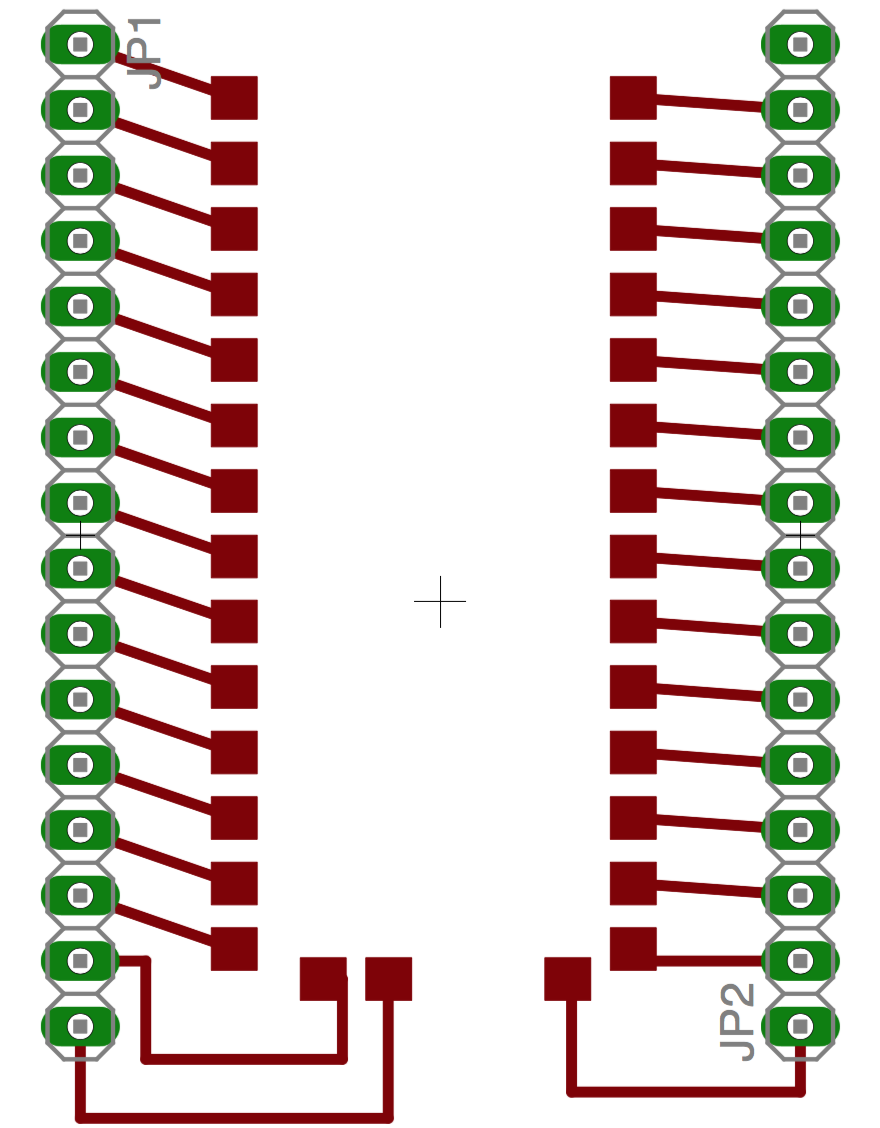
\includegraphics[scale=0.4]{kh3-receiver-breakout.png}
	\caption{R.F. Receiver/Antenna PCB Schematic\label{fig:receiver-breakout}}
\end{figure}

\begin{figure} [H]
	\centering
	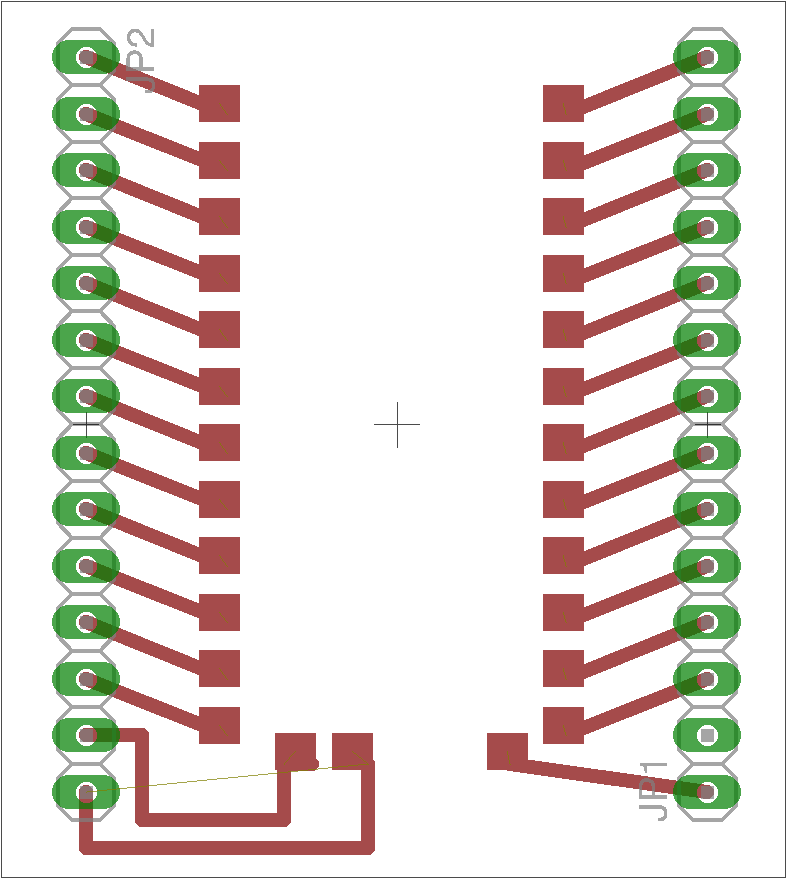
\includegraphics[scale=1.8]{kh3-transmitter-breakout.png}
	\caption{R.F. Receiver/Antenna PCB Schematic\label{fig:receiver-breakout}}
\end{figure}

\section{Ethical Considerations} 
The following ethical considerations refer to the IEEE Code of Ethics\cite{IEEE}.

\textit{"1. To accept responsibility in making decisions consistent with the safety, health, and welfare of the public, and to disclose promptly factors that might endanger the public or the environment"} \\
\textit{"9. To avoid injuring others, their property, reputation, or employment by false or malicious action"}

Our project fully acknowledges the danger of lasers, and in the design review calculated an NOHD (Nominal Ocular Hazard Distance) of $1.25m$. Another aspect of the project that could endanger the public is the misuse of an IFF system. We want to be clear that just because a target doesn't acknowledge as "friendly" does NOT mean that the target is dangerous. As always, anyone wielding a firearm should consider both the target and the area behind the target before firing. This system is meant to supplement, not replace, good judgment.  

\textit{"2. To avoid real or perceived conflicts of interest whenever possible, and to disclose them to affected parties when they do exist"}

Our project may contain conflicts of interest in that two opposite sides of a combat scenario could use this technology. We would disclose this information to both sides. It is our hope that this technology will reduce the amount of friendly fire casualties, regardless of allegiance. 

\textit{"3. To be honest and realistic in stating claims or estimates based on available data"}

We will always be honest with the capabilities of this system. To skew the capabilities could put infantry and non-combatants in danger. 

\textit{"5. To improve the understanding of technology; its appropriate application, and potential consequences"}\\
\textit{"6. To maintain and improve our technical competence and to undertake technological tasks for others only if qualified by training or experience, or after full disclosure of pertinent limitations"}

The entire purpose of senior design is to meet these requirements. As college students, we aspire to improve ours, and other's, understanding of technology. We also fully acknowledge limitations of our abilities and will supplement with help from the course staff. 

\textit{"7. To seek, accept, and offer honest criticism of technical work, to acknowledge and correct errors, and to credit properly the contributions of others"}

We are always willing to have a dialog with those interested in are work. We also seek to correct any errors so that the project meets all requirements. In building any project, one relies heavily on work already done by others; it is important to give credit where it is due. 

\section{Conclusion}
Over the next few weeks, there are several large tasks that must be completed: 
\begin{enumerate}
	\item Build an adjustable focus $5mW$ red laser
	\item Solder, debug, and verify the friendly target pcb
	\item Write software to keep a system clock
	\item Write software to process incoming id signals and produce ack
	\item Migrate to a final friendly target pcb
	\item Perform requirements verification on both final units
\end{enumerate}

Software will likely be an ongoing process throughout the next weeks. I plan on building the laser in a week, after receiving the parts. The soldering and debugging of the friendly target pcb should take, at most, 2 weeks. 

While the team has had some setbacks, including incorrect part orders and shorted/fried parts, we are still on schedule to finish the project by demonstration. The workload over the next few weeks will be heavy, but I am confident we can finish the project. 

After having worked on a large-scale project in Cubesat together, Eric and I make a formidable team. As such, we have done a fantastic job splitting the work evenly. Both of us pick tasks to work on, and report progress to each other often. The estimated 13 hours/week was optimistic. For all of the progress shown in this report, it has taken closer to 20 hours per week, sometimes less sometimes more. My hope is that, in putting this work forward now, the workload will diminish later in the semester. In any case, I would rather be finished early than be rushing to complete a large project in the last few weeks of the semester. 


%SECTION - References
\bibliographystyle{IEEE_ECE}
% include the BibTex file here to build reference
\bibliography{Citations}\addcontentsline{toc}{section}{Reference}
\end{spacing}
\end{document}

